\documentclass[tesis.tex]{subfiles}
\begin{document}
    
\section{Discussion}

Cosas a explicar (discutir que hubiese pasado si esto es diferente).

\textit{Para mí el capitulo fundamental. Los resultados son analizados en detalle, pudiendo incorporar análisis adicionales que no estaban inicialmente en la metodología, como para entender, entre otras cosas, la sensibilidad de los resultados ante parámetros por ejemplo. O la comparación con resultados de otros estudios, o conocimiento existente. En este capítulo se debe entender si lo que se hizo es útil o no.}

\subsection{Estuarine structure and morphology}

During the winter of 2012 Pescadero estuary received less freshwater inflow compared to other months throughout the year, leading the inlet to disconnect from the ocean. Pescadero during its closed state function as a stratified coastal lagoon with river runoff forming a surface layer of fresh water and occasionally having tidal inflows of saline water. The orientation of the bay and the shallowness result in the exposure of all the water column to the wind stress events. In this regard, Pescadero shares many physical traits with other bar-built estuaries where the local wind forcing is the dominant driver.\\

Apart from the stratification, there is an along-estuary density gradient between the outlet of the creek and the mouth, due to the constant discharge of freshwater. Near the mouth the upper layer is thinner than in the creek's outlet, probably because the salinity is higher in the mouth due to the waves that are overtopping the sandbar along with upstream continuous freshwater input.\\

The present study analysis reported that the major driver of mixing is wind stress and the major driver of water level variability is freshwater inflow, even in periods when is very low. In the next sections we are going to discuss the role of other factors that affect Pescadero and its importance in stratification and water level.\\

\subsection{Analysis methods}

Wind and estuarine velocities were axis-rotated in the direction of maximum variance of water currents (See Fig. \ref{fig:rotacion}, Section \ref{Estuary_currents}). This puts the main focus in the estuary currents instead of the wind velocity, but in this particular case, both, wind and water velocities, have a similar principal direction, so it wouldn't be a big difference between each option.\\

We adjusted the first cell of the ADCP data by a visual inspection, using the blank space given by the ADCP, that was 0.71 m, and overlapping it with the CTD data on the same location DC. This comparison gave us the value of 0.91 m for the first cell location, which is a merely estimation, so it could have been a different value, bigger or smaller depending in how we had place the overlapping. This does not affect velocity values, but we have to consider it for the positions of the layers or for the profiles, but it does not make an important change in the analysis.\\

The closed state definition was set in a range of depth's change in time values with a 10 hour frame. The frame was selected by trial and error based on the timescale we were working on and it could change depending on the period in which the data was collected and in the data collection frequency. Also we have to consider that the opening and closures do not happen on an instant, but in a process that could last from minutes to hours, so it could be considered any instant during that process.\\ 

In this study we did not considered temperature and evaporation factors. We considered that the efect of temperature was not important due to the haline stratification that dominated the estuary, but it could be studied in greater depth in future analyzes carried out in Pescadero. Also, we didn't consider evaporation as a factor in depth changes because we are studing an estuary with small area and as it was winter time the air temperature was not too hight to cause mayor impacts.\\

To calculate wind stress we used a drag coefficient defined by \cite{large1981open}, but according to \cite{paugam2021wind} the drag coefficient $C_D$ can be difficult to estimate in shallow water, so we have to consider the obtained $C_D$ as an aproximation in wind stress and everything calculated with that coefficient. In future studies there could be used other drag coefficients to observe if there is a big difference in wind stress and other indices obtained with $C_D$.\\

The Wedderburn number was obtained with the equation for a rectangular basin defined by \cite{Monismith1985}, so it is showing us an approximated value. Despite this, it is still a good indicator to estimate the behavior of the stratification to the wind stress. We could try in future research more adapted Wedderburn numbers to Pescadero basin and compare the results with the obtained in this study.\\

The frequency spectral analysis only show a general view of the most important frequencies in the dataset, but does not show the specific time when this happens. This make it an special tool to detect fequency peaks and contrasts different datasets.\\

\subsection{Changes in Pescadero over time}

\subsection{Wind stress mixing}

Sporadic abrupt changes in density along the water column in different locations were apparent during the periods of closed state. This sudden changes indicate that they were not caused by gradual processes, but rather resulted from sporadic events that are attributed to the effects of wind stress present at the same time as the density changes. After this events, density did not return to its original values from before the event so mixing was present in the three studied locations.\\

Fig. \ref{fig:perfiles2} is showing density profiles in the studied locations before (in red) and after (in cyan) a big wind event, showing a difference in the density values specially in the bottom where there is a decrease in density. Buoyancy frequency showed a decreased after the wind event meaning a change in stratification, same as potential energy anomaly in Fig. \ref{fig:phi}. Also Fig. \ref{fig:diff} $\Delta \rho/\Delta z$ is showing a decrease in stratification between before and after big wind events, only observing this abrupt change twice, one time during each closed state period.\\

We chose to obtain a range of values for the Wedderburn number as we did not know the exact placement of the pycnocline. Due to the constant freshwater inflow, the stratification of the estuary is changing over time, which means the surface layer is also changing its thickness. The range limits of W were obtained as a function that depends directly on the water level. We assumed the density interface theoretically reaches the upwind surface at W = 1, so if the full range of W goes lower that value we will consider it a full upwelling. During a full upwelling, if we consider a linear tilt, the range lower limit reaches the surface, different for the partial upwelling, where just the upper limit reach the surface. The main difference between both events of upwelling is that the full one is changing the density structure and the other one isn't. We can observe this in Fig. \ref{fig:phi} where the potential energy anomaly after the partial upwelling events is not changing. During the upwelling events there is the presence of baroclinic pressure gradients which increase with a lower W, so during the partial upwelling events, the gradients are not enough to mix the water column and change the stratification structure.\\

On the other hand, we observed surface fluctuations during the wind events, which are noticeable in the wavelet analysis in Fig. \ref{fig:surf2}. Also, there is a small relation between wind and depth density frequencies (Fig. \ref{fig:freq}) around a period of 200 min.\\

The complex current and isotherm patterns observed during relaxation are consistent with theory

The inconsistency in (lag) the apparent relaxation time scale would seem to imply the presence of baroclinic currents

\subsection{Wind-driven circulation}

During and after wind events there were observed circulation processes that are indicating how the layers of the estuary behave. We already noticed that the main driver of changes in velocity in the estuary is wind stress. In Fig. \ref{fig:velwind} we observed with more detail the circulation occurring around the first wind event of the second period. We observed that the estuary had some circulation occurring before the event, when there is no wind stress, due to the constant freshwater inflow that is present in Pescadero. This velocity is positive (streamflow direction) and is at the superior layer detected by the ADCP. Also, before the wind event, with $\tau_w =0$, there was a negative velocity at the top of the range occuring at the same time of a detected wave overtopping event, meaning that the waves were creating a small circulation in the surface of the estuary that was overlaping the discharge velocity.\\

\begin{figure}[h!]
    \centering
    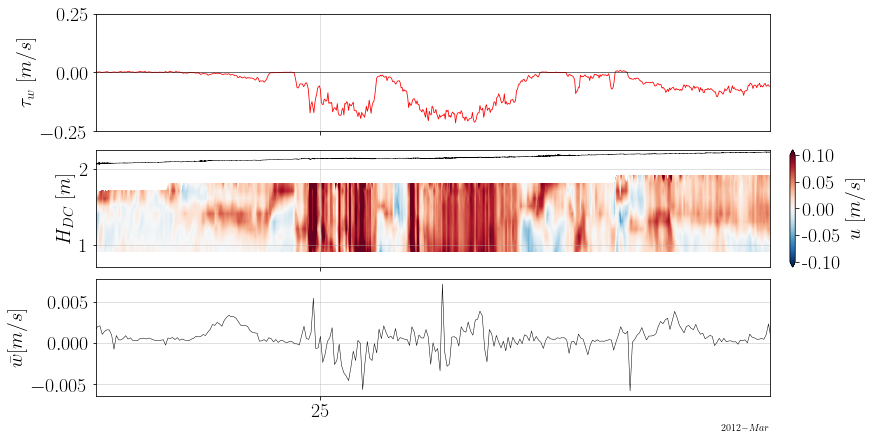
\includegraphics[width=\textwidth]{Imagenes/vel_wind.png}
    \caption{Along-estuary velocity }
    \label{fig:velwind}
\end{figure}

During the wind event we observed an increase in velocity in positive direction, while the wind stress is negative. The literature says that a stratified waterbody that is subjected to a surface stress has its surface layer circulating with the same direction of the wind with a set-up of the free surface at the leeward zone, depressing the pycnocline and resulting in set-down at the wind leeward shore and a circulation of the lower layer in the opposite direction of the wind \citep{Katopodes2018}. Despite the last statement we observed in Fig. \ref{fig:velwind} the velocity during a wind event is in the opposite direction of the wind. This is due to the range of available data from the ADCP, which starts measuring at 0.91 m and doesn't work near the surface, not showing the surface layer circulation and skipping the part where the velocity is at the same direction of the wind. Also, when the wind blows, the upper layer moves towards the surface and upstream moving away from detected range (Fig. \ref{fig:adcp}) making the upper layer thinner at the DC location.\\

\begin{figure}[h!]
    \centering
    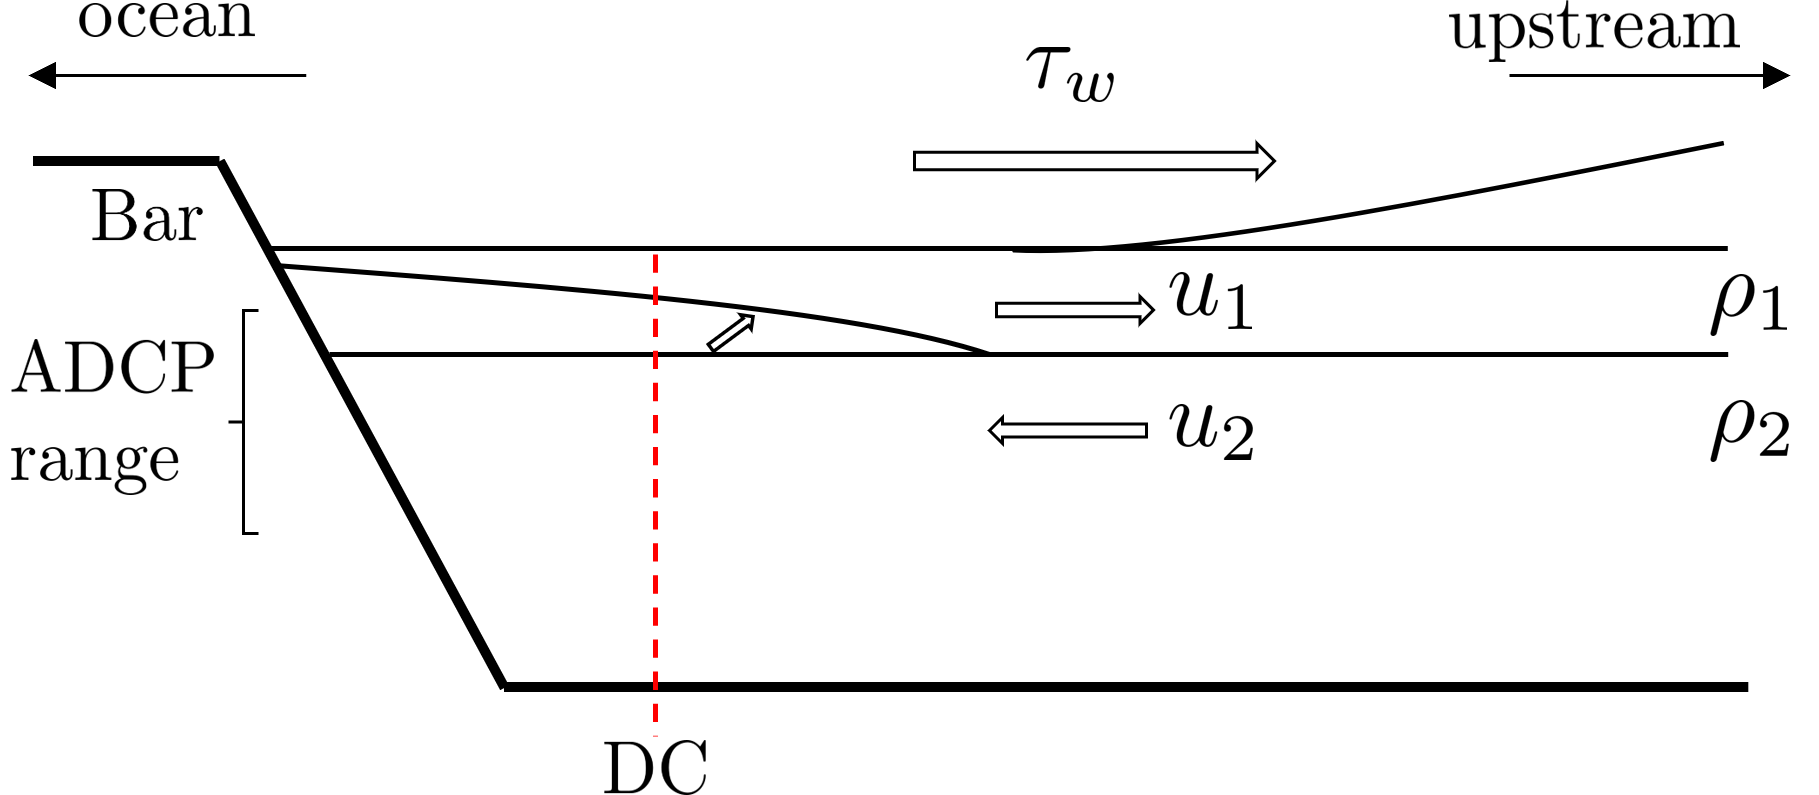
\includegraphics[width=0.6\textwidth]{Imagenes/ADCP_range.png}
    \caption{Scheme of the pycnocline tilt in an idealized estuary with an example of the detected ADCP range in Pescadero.}
    \label{fig:adcp}
\end{figure}

Following the relaxation of the winds, the baroclinic pressure return the estuary to its original state generating currents which are present mostly at the lower layers of the ADCP range (Fig. \ref{fig:velwind}). We observed negative velocities after the first relaxation between the two wind increases. First negative velocities were present at the lower part, representing the return of the middle layer to its equilibrium position, while at the top velocities were positive, maybe showing the surface layer dynamics. After less than two hours there was a flip on the dynamics, at the upper part positive and at the lower negative, meaning probably a seiche in the estuary.\\

\newpage
\begin{figure}[h!]
    \centering
    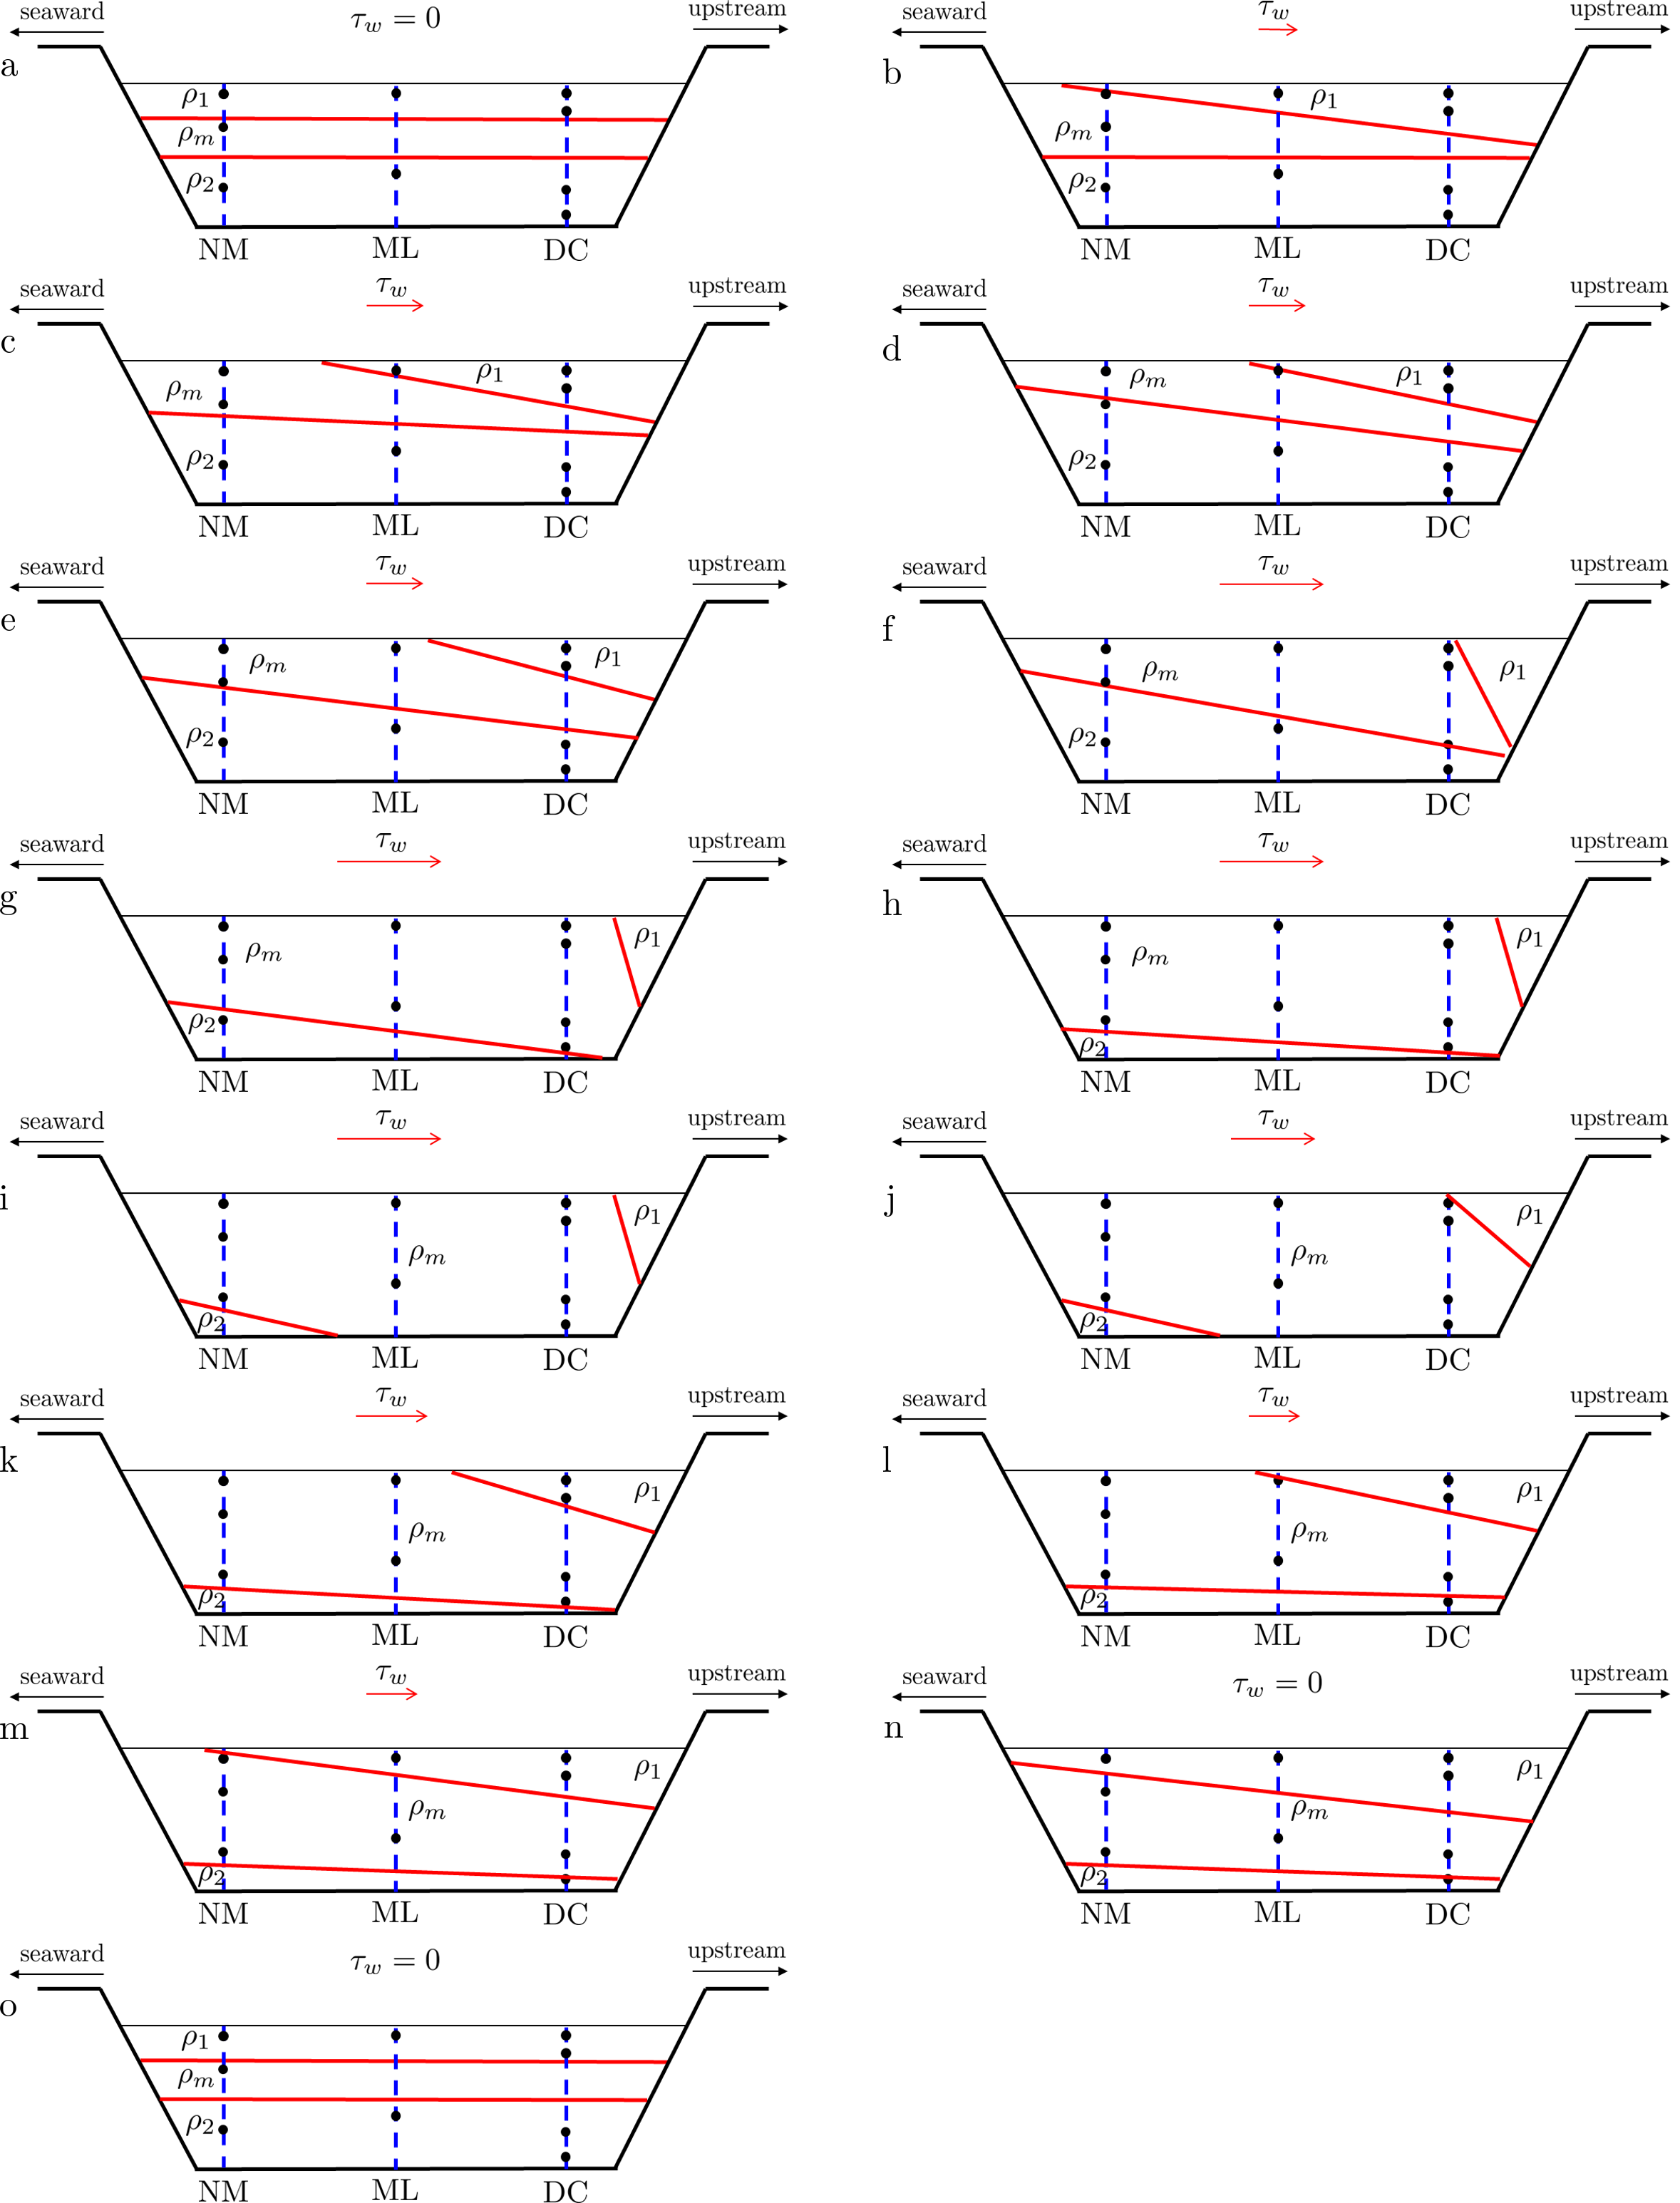
\includegraphics[width=0.95\textwidth]{Imagenes/wind_event.png}
    \caption{Wind event}
    \label{fig:wevent}
\end{figure}

\newpage
\begin{figure}[h!]
    \centering
    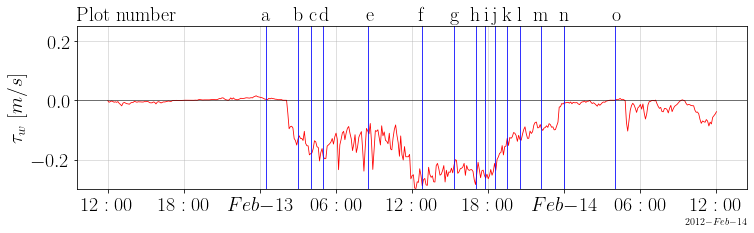
\includegraphics[width=0.95\textwidth]{Imagenes/wind_event2.png}
    \caption{Wind event}
    \label{fig:wevent2}
\end{figure}

After the second increase was observed a similar dynamic than after the first increase, but we didn't observe the flip happen. We observed that at the same time there was a wave overtopping event that probably affected the recirculation, but as it did not cause the same effect than before of negative velocities at the top its possible that it is not affecting the velocities with the same magnitude or it is overlapping the velocities of the relaxation changing its behaviour. Other reason for the flip not happening is that the oscillation hadn't enough amplitude, so the seiche didn't happen.\\

Also, we studied the first wind event of the first period using the densities at locations NM, ML and DC. At Fig. \ref{fig:wevent} we plotted the behavior of the layers according to the densities at different instants of time showed at Fig. \ref{fig:wevent2}. The sensors were centered at the horizontal and had a proporcional distance to reality in the vertical for an easier estimation of the layers with the available information. During the wind event the surface layer is moving landward due to the wind stress going in that direction, not being shown by any sensor at the biggest wind stress. The middle layer was occupying all the water column for all the sensors during the peak of the wind event. The lower layer had an incertain movement, but we drawed it as the sensors were showing it, going in the same direction of the middle layer, not having the behavior of a third layer.\\

\subsection{Freshwater input}

The density time-series were showing a density decrease in time, specially at the bottom layer in NM and ML (Fig. \ref{fig:dens}), in DC we also observed a decrease but not in the deepest layer, in which we observed a light increase of density in the first period. The density decrease in time indicates a constant freshwater input. The parameter $\Delta \rho / \Delta z$ is also slowly changing in time, fact that is not observable at Fig. \ref{fig:diff}, but what is clear is the change between before and after a wind event that is decreasing over time, showing that wind stress is affecting each time less the estuarine structure. The last statement is also noticeable in Wedderburn number (Fig. \ref{fig:wedd}) where we observe in the last wind events W barely get closed to the threshold.\\

The destratification of the estuary could be a result of the freshwater constant input that is changing the density structure continously in time. Also, it could be a result of the mixing that triggers during the discharge increse in storm events due to the water enters with more velocity, which can induce interfacial instability \citep{Katopodes2018}. The last one is only reflected in the surface (Fig. \ref{fig:surf}) and is not very clear in the density, specially as it happens at the same time a wind event in the first period and a wave overtopping event in the second period. The last two ways of destratification are working together with wind stress to change the estuarine density structure. As the estuary has a constant decrease in density, freshwater inflow is affecting the estuary, and as density changes occur during wind events while there is not a discharge increase, wind is important in the lagoon. In addition, it is possible that the abrupt changes in the amount of incoming flow generate mixing, although there is not enough evidence to say that this is happening.\\

Like we said before, the two registered freshwater inflow increases happened with other events at the same time, the first one during a wind event and the other while there was wave overtopping. That is why we cannot attribute the changes observed in $\hat{H}$, $dh/dt$ or $\Delta \hat{H}/\Delta x$ exclusively to discharge increase. In Fig. \ref{fig:qh} we observe discharge versus the water level and the level change in time. The first one had a strong correlation until $Q$ started decreasing while $H_{DC}$ still increase. The second plot also has some correlation, but we observe is not constant in time, so $Q$ did not affect constantly the same at the water level increase rate, but still there is a strong relationship between them.\\

Fig. \ref{fig:mix_q} is showing the second discharge increase that happened at the same time a wave overtopping event. We observed surface fluctuations in $\hat{H}$ while it was increasing and the $\Delta \rho/\Delta z$ increasing also. We observed that $\hat{H}$ changed when wave overtopping started and $\Delta \rho/\Delta z$ when $Q$ increased, but the latter incre

\begin{figure}[h!]
    \centering
    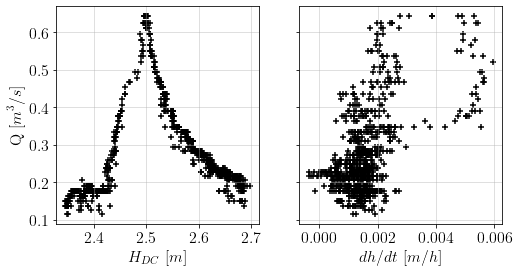
\includegraphics[width=0.8\textwidth]{Imagenes/qh.png}
    \caption{Discharge versus estuary height and discharge versus the height change in a 10-hour-frame for the period between February 11th and February 20th.}
    \label{fig:qh}
\end{figure}


\begin{figure}[h!]
    \centering
    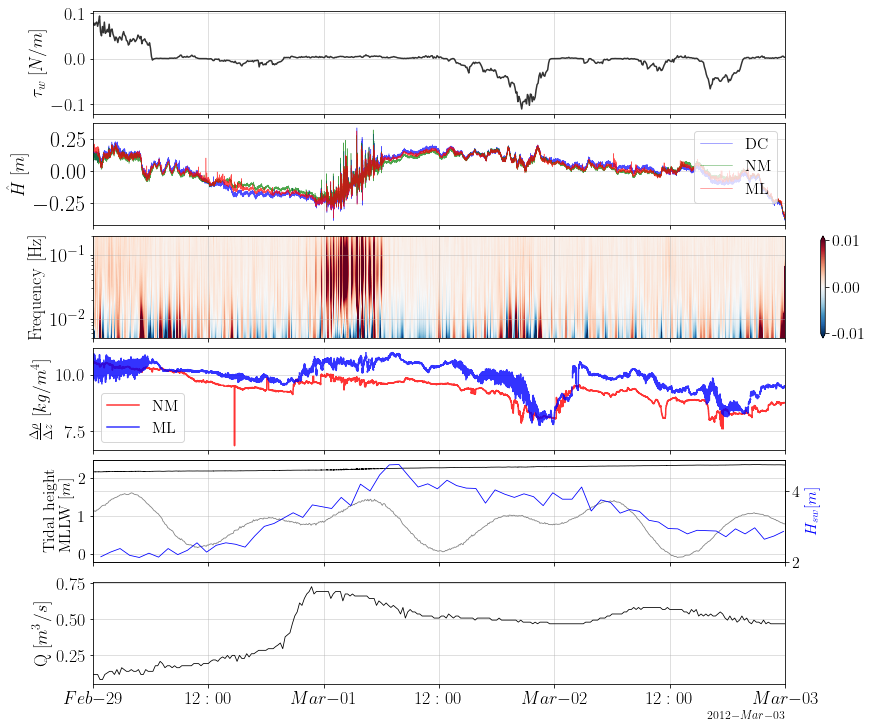
\includegraphics[width=\textwidth]{Imagenes/mix_q.png}
    \caption{ddfsdfsdf }
    \label{fig:mix_q}
\end{figure}

\subsection{Wave overtopping}

pasa cuando la marea esta subiendo 
provoca cambios en las velocidades superficiales


- There could be presence of density increase due to wave overtopping 

- In results section we observed some small changes in desnity after wave overtopping 

- Menos en Dc que vimos cambios en el tiempo en el primer periodo.

* Graficos de tau, rho DC fondo, wavelet, d rho/dt 10-hour-frame, Tide/Pdo/Hsw

Why during wave overtopping the bottom of NM increase and then go to normal
explain the  continuous increase in DC at the bottom

The wavelet analysis shows high-frequency waves when that occurs (Figure 3-D and 3-H), but it could be hiding some insignificant wave overtop events.

- Por otro lado, podría haber mezcla en el estuario debido a la entrada turbulenta de las olas sobre la barra de arena.

- Esto se podría atribuir a que cuando hay wave overtopping se observan fluctuaciones en la superficie (H hat, dh/dt, DH hat/Dx, Q), además de los pequeños cambios observados en la densidad

- igual que para el Caso del caudal las surface fluctuations Pueden Ser indicadores de que hay mezcla

- no hay evidencia que lo respalde.

\begin{figure}[h!]
    \centering
    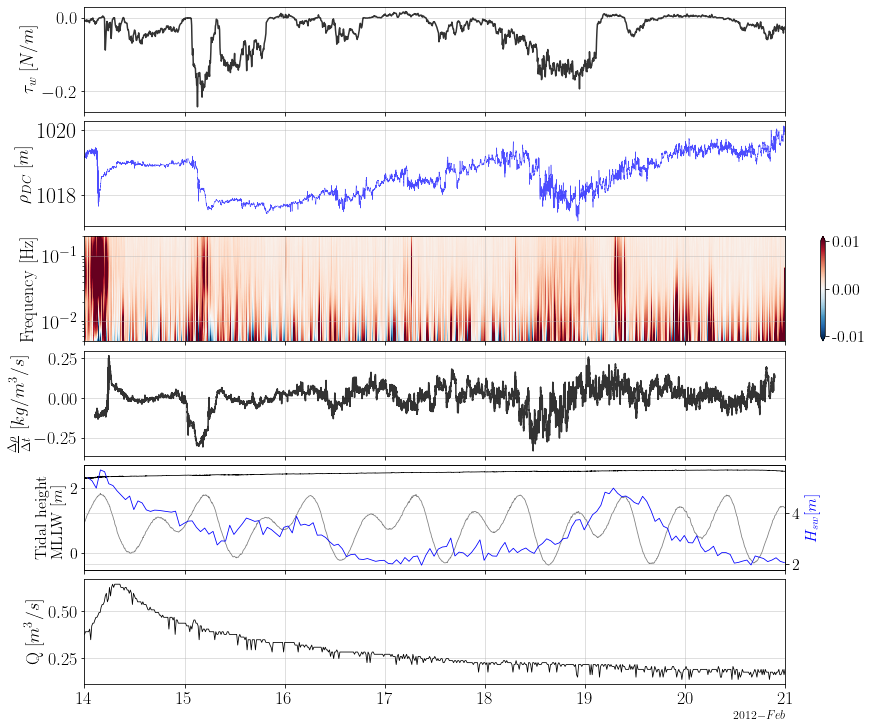
\includegraphics[width=\textwidth]{Imagenes/mix_wo.png}
    \caption{ddfsdfsdf }
    \label{fig:mix_wo}
\end{figure}


\end{document}